\section{Результаты}
\subsection{Выборочные коэффициенты корреляции}
\begin{table}[H]
	\centering
	\begin{tabular}{| c | c | c | c |}
		
		\hline
		$\rho = 0$ & $r$      & $r_S$  & $r_Q$ \\
		\hline
		$E(z)$    & 0.002 & 0.002 & 0.0   \\
		$E(z^2)$  & 0.028 & 0.026 & 0.04  \\
		$D(z)$    & 0.054 & 0.053 & 0.053 \\
		\hline
		$\rho = 0.5$ & $r$      & $r_S$  & $r_Q$ \\
		\hline
		$E(z)$       & 0.506 & 0.481 & 0.4   \\
		$E(z^2)$    & 0.256 & 0.232 & 0.16  \\
		$D(z)$      & 0.028 & 0.031 & 0.045 \\
		\hline
		$\rho = 0.9$ & $r$      & $r_S$  & $r_Q$ \\
		\hline
		$E(z)$       & 0.905 & 0.879 & 0.8   \\
		$E(z^2)$    & 0.819 & 0.773 & 0.64  \\
		$D(z)$      & 0.002 & 0.004 & 0.029 \\
		\hline
		
	\end{tabular}{}
	\caption{Двумерное нормальное распределение, n = 20}
	\label{tab:n20}
\end{table}


\begin{table}[H]
	\centering
	\begin{tabular}{| c | c | c | c |}
		
		\hline
		$\rho = 0$ & $r$      & $r_S$  & $r_Q$ \\
		\hline
		$E(z)$     & -0.002 & -0.004 & 0.0   \\
		$E(z^2)$  & 0.007  & 0.007  & 0.004 \\
		$D(z)$    & 0.017  & 0.017  & 0.017 \\
		\hline
		$\rho = 0.5$ & $r$      & $r_S$  & $r_Q$ \\
		\hline
		$E(z)$       & 0.507 & 0.488 & 0.333 \\
		$E(z^2)$    & 0.257 & 0.238 & 0.111 \\
		$D(z)$      & 0.009 & 0.01  & 0.015 \\
		\hline
		$\rho = 0.9$ & $r$      & $r_S$  & $r_Q$ \\
		\hline
		$E(z)$       & 0.901 & 0.885 & 0.733 \\
		$E(z^2)$    & 0.812 & 0.783 & 0.538 \\
		$D(z)$      & 0.001 & 0.001 & 0.008 \\
		\hline
		
	\end{tabular}{}
	\caption{Двумерное нормальное распределение, n = 60}
	\label{tab:n60}
\end{table}



\begin{table}[H]
	\centering
	\begin{tabular}{| c | c | c | c |}
		
		\hline
		$\rho = 0$ & $r$      & $r_S$  & $r_Q$ \\
		\hline
		$E(z)$     & 0.002 & -0.0  & 0.0   \\
		$E(z^2)$  & 0.005 & 0.004 & 0.006 \\
		$D(z)$    & 0.011 & 0.011 & 0.01  \\
		\hline
		$\rho = 0.5$ & $r$      & $r_S$  & $r_Q$ \\
		\hline
		$E(z)$       & 0.5   & 0.477 & 0.32  \\
		$E(z^2)$    & 0.25  & 0.228 & 0.102 \\
		$D(z)$     & 0.006 & 0.006 & 0.009 \\
		\hline
		$\rho = 0.9$ & $r$      & $r_S$  & $r_Q$ \\
		\hline
		$E(z)$       & 0.901 & 0.889 & 0.72  \\
		$E(z^2)$    & 0.812 & 0.791 & 0.518 \\
		$D(z)$      & 0.0   & 0.001 & 0.005 \\
		\hline
		
	\end{tabular}{}
	\caption{Двумерное нормальное распределение, n = 100}
	\label{tab:n100}
\end{table}


\begin{table}[H]
	\centering
	\begin{tabular}{| c | c | c | c |}
		
		\hline
		$size = 20$ & $r$      & $r_{S}$ & $r_{Q}$ \\
		\hline
		$E(z)$       & 0.793 & 0.756 & 0.6   \\
		$E(z^2)$    & 0.628 & 0.572 & 0.36  \\
		$D(z)$       & 0.009 & 0.014 & 0.037 \\
		\hline
		$size = 60$ & $r$      & $r_{S}$ & $r_{Q}$ \\
		\hline
		$E(z)$       & 0.793 & 0.773 & 0.6   \\
		$E(z^2)$    & 0.629 & 0.597 & 0.36  \\
		$D(z)$      & 0.002 & 0.003 & 0.011 \\
		\hline
		$size = 100$ & $r$      & $r_{S}$ & $r_{Q}$ \\
		\hline
		$E(z)$        & 0.792 & 0.774 & 0.56  \\
		$E(z^2)$     & 0.627 & 0.599 & 0.314 \\
		$D(z)$        & 0.001 & 0.002 & 0.007 \\
		\hline
		
	\end{tabular}{}
	\caption{Смесь нормальных распределений}
	\label{tab:mix_normal}
\end{table}
\subsection{Эллипсы рассеивания}
\noindent Для уравнения эллипса выбиралась константа равная $const = 2 \cdot (2 \cdot \sigma)$

\begin{figure}[H]
	\centering
	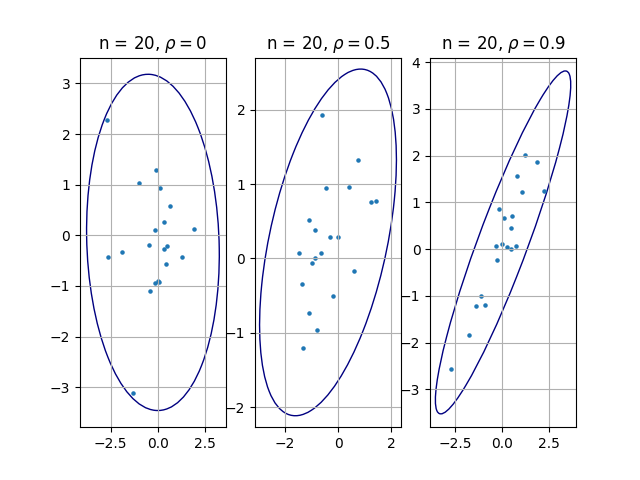
\includegraphics[width = 13cm, height = 8cm]{resources/5_20.png}
	\caption{Двумерное нормальное распределение, $n$ = 20}
	\label{fig:n20}
\end{figure}

\begin{figure}[H]
	\centering
	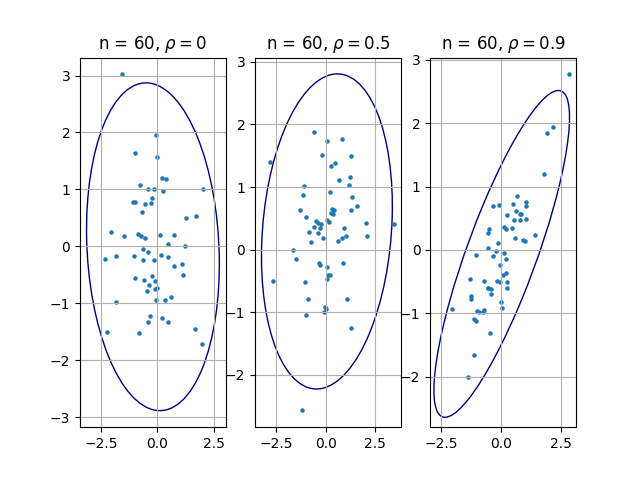
\includegraphics[width = 13cm, height = 8cm]{resources/5_60.png}
	\caption{Двумерное нормальное распределение, $n$ = 60}
	\label{fig:n60}
\end{figure}

\begin{figure}[H]
	\centering
	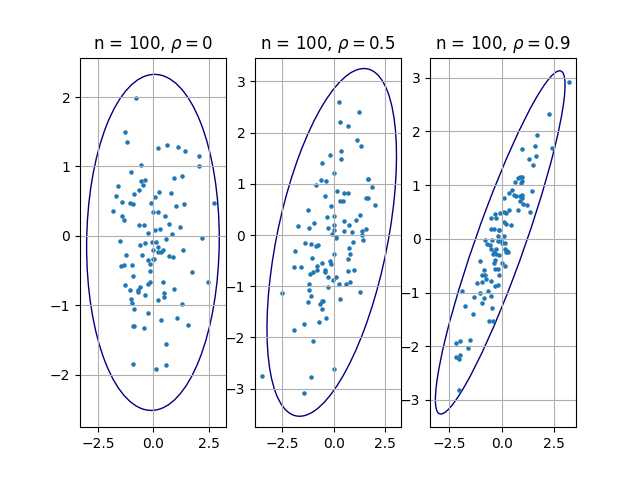
\includegraphics[width = 13cm, height = 8cm]{resources/5_100.png}
	\caption{Двумерное нормальное распределение, $n$ = 100}
	\label{fig:n100}
\end{figure}
\subsection{Оценки коэффициентов линейной регрессии}

\noindent Метрика удаленности: $distance = \sum_{i=0}^{n}(y_{model}[i]-y_{regr}[i])^2$
\subsubsection{Выборка без возмущений}
\begin{enumerate}
	\item{Критерий наименьших квадратов:}
	$\hat{a}\approx 2.07$, $\hat{b}\approx 1.82$
	\item{Критерий наименьших модулей:}
	$\hat{a}\approx 2.11$, $\hat{b}\approx 1.75$
\end{enumerate}
\begin{figure}[H]
	\centering
	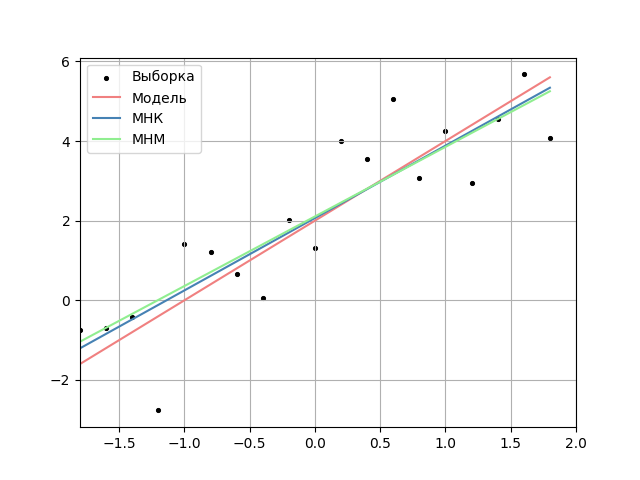
\includegraphics[width = 10cm, height = 8cm]{resources/6_1.png}
	\caption{Выборка без возмущений}
	\label{w/o_pert}
\end{figure}

\subsubsection{Выборка с возмущениями}
\begin{enumerate}
	\item{Критерий наименьших квадратов:}
	$\hat{a}\approx 2.13$, $\hat{b}\approx 0.53$
	\item{Критерий наименьших модулей:}
	$\hat{a}\approx 1.97$, $\hat{b}\approx 1.93$
\end{enumerate}
\begin{figure}[H]
	\centering
	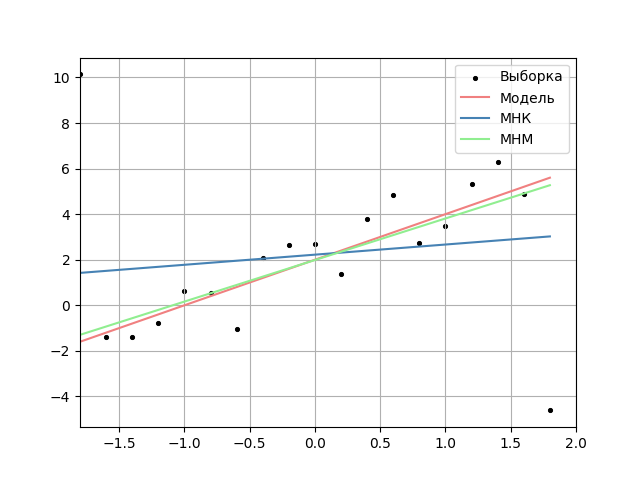
\includegraphics[width = 10cm, height = 8cm]{resources/6_2.png}
	\caption{Выборка с возмущениями}
	\label{w_pert}
\end{figure}
\subsection{Проверка гипотезы о законе распределения генеральной совокупности. Метод хи-квадрат}

\noindent Метод максимального правдоподобия:
\newline
$\hat{\mu} \approx -0.23, \hat{\sigma} \approx 1.03$
\newline
Критерий согласия $\chi^{2}$:
\newline
Количество промежутков $k = 8$
\newline
Уровень значимости $\alpha$= 0.05
\newline
Тогда квантиль $\chi^{2}_{1-\alpha}(k-1)$ = $\chi^{2}_{0.95}(7)$. $\chi^{2}_{0.95}(7) \approx 14.07$. 
\begin{table}[H]
	\centering
	\begin{tabular}{| c | c | c | c | c | c | c |}
		\hline
		$i$ & $limits$         &   $n_i$ &    $p_i$ &   $np_i$ &   $n_i - np_i$ &   $\frac{(n_i-np_i)^2}{np_i}$ \\
		\hline
		1 & ($-\infty$, -1.1] &    23 & 0.1357 &  13.57 &         9.43 &                        6.56 \\
		2 & [-1.1, -0.73]  &    11 & 0.096  &   9.6  &         1.4  &                        0.2  \\
		3 & [-0.73, -0.37] &    10 & 0.1253 &  12.53 &        -2.53 &                        0.51 \\
		4 & [-0.37, 0.0]   &    13 & 0.1431 &  14.31 &        -1.31 &                        0.12 \\
		5 & [0.0, 0.37]    &    14 & 0.1431 &  14.31 &        -0.31 &                        0.01 \\
		6 & [0.37, 0.73]   &    13 & 0.1253 &  12.53 &         0.47 &                        0.02 \\
		7 & [0.73, 1.1]    &     5 & 0.096  &   9.6  &        -4.6  &                        2.21 \\
		8 & [1.1, $+\infty$)   &    11 & 0.1357 &  13.57 &        -2.57 &                        0.49 \\
		\sum & -              &   100 & 1      & 100    &        -0    &                       10.11 \\
		\hline
	\end{tabular}
	\caption{ Вычисление $\chi^{2}_{B}$ при проверке гипотезы $H_{0}$ о нормальном законе распределения $N(x,\hat{\mu}, \hat{\sigma})$}
	\label{tab:normal_chi_2}
\end{table} 

\noindent Сравнивая $\chi^{2}_{B} = 10.11$ и $\chi^{2}_{0.95}(7) \approx 14.07$, видим, что $\chi^{2}_{B} < \chi^{2}_{0.95}(7)$.
\\

\begin{table}[H]
	\centering
	\begin{tabular}{| c | c | c | c | c | c | c |}
		\hline
		$i$ & $limits$         &   $n_i$ &    $p_i$ &   $np_i$ &   $n_i - np_i$ &   $\frac{(n_i-np_i)^2}{np_i}$ \\
		\hline
		1 & ($-\infty$, -1.1] &     1 & 0.1357 &   2.71 &        -1.71 &                        1.08 \\
		2 & [-1.1, -0.37]  &     3 & 0.2213 &   4.43 &        -1.43 &                        0.46 \\
		3 & [-0.37, 0.37]  &    12 & 0.2861 &   5.72 &         6.28 &                        6.89 \\
		4 & [0.37, 1.1]    &     2 & 0.2213 &   4.43 &        -2.43 &                        1.33 \\
		5 & [1.1, $+\infty$)   &     2 & 0.1357 &   2.71 &        -0.71 &                        0.19 \\
		\sum & -              &    20 & 1      &  20    &        -0    &                        9.94 \\
		\hline
	\end{tabular}
	\caption{ Вычисление $\chi^{2}_{B}$ при проверке гипотезы $H_{0}$ о законе распределения $L(x,\hat{\mu}, \hat{\sigma})$, $n=20$}
	\label{tab:laplace_chi_2}
\end{table}
\noindent Сравнивая $\chi^{2}_{B} = 9.94$ и $\chi^{2}_{0.95}(4) \approx 9.49$, видим, что $\chi^{2}_{B} > \chi^{2}_{0.95}(4)$.

\begin{table}[H]
	\centering
	\begin{tabular}{| c | c | c | c | c | c | c |}
		\hline
		$i$ & $limits$         &   $n_i$ &    $p_i$ &   $np_i$ &   $n_i - np_i$ &   $\frac{(n_i-np_i)^2}{np_i}$ \\
		\hline
		1 & ($-\infty$, -1.1] &     4 & 0.1357 &   2.71 &         1.29 &                        0.61 \\
		2 & [-1.1, -0.37]  &     4 & 0.2213 &   4.43 &        -0.43 &                        0.04 \\
		3 & [-0.37, 0.37]  &     5 & 0.2861 &   5.72 &        -0.72 &                        0.09 \\
		4 & [0.37, 1.1]    &     2 & 0.2213 &   4.43 &        -2.43 &                        1.33 \\
		5 & [1.1, $+\infty$)   &     5 & 0.1357 &   2.71 &         2.29 &                        1.93 \\
		\sum & -              &    20 & 1      &  20    &        -0    &                        4    \\
		\hline
	\end{tabular}
	\caption{ Вычисление $\chi^{2}_{B}$ при проверке гипотезы $H_{0}$ о законе распределения $U(x,\hat{\mu}, \hat{\sigma})$, $n=20$}
	\label{tab:uniform_chi_2}
\end{table}

\noindent Сравнивая $\chi^{2}_{B} = 4$ и $\chi^{2}_{0.95}(4) \approx 9.49$, видим, что $\chi^{2}_{B} < \chi^{2}_{0.95}(4)$.

\subsection{Доверительные интервалы для параметров нормального распределения}
\begin{figure}[H]
	\centering
	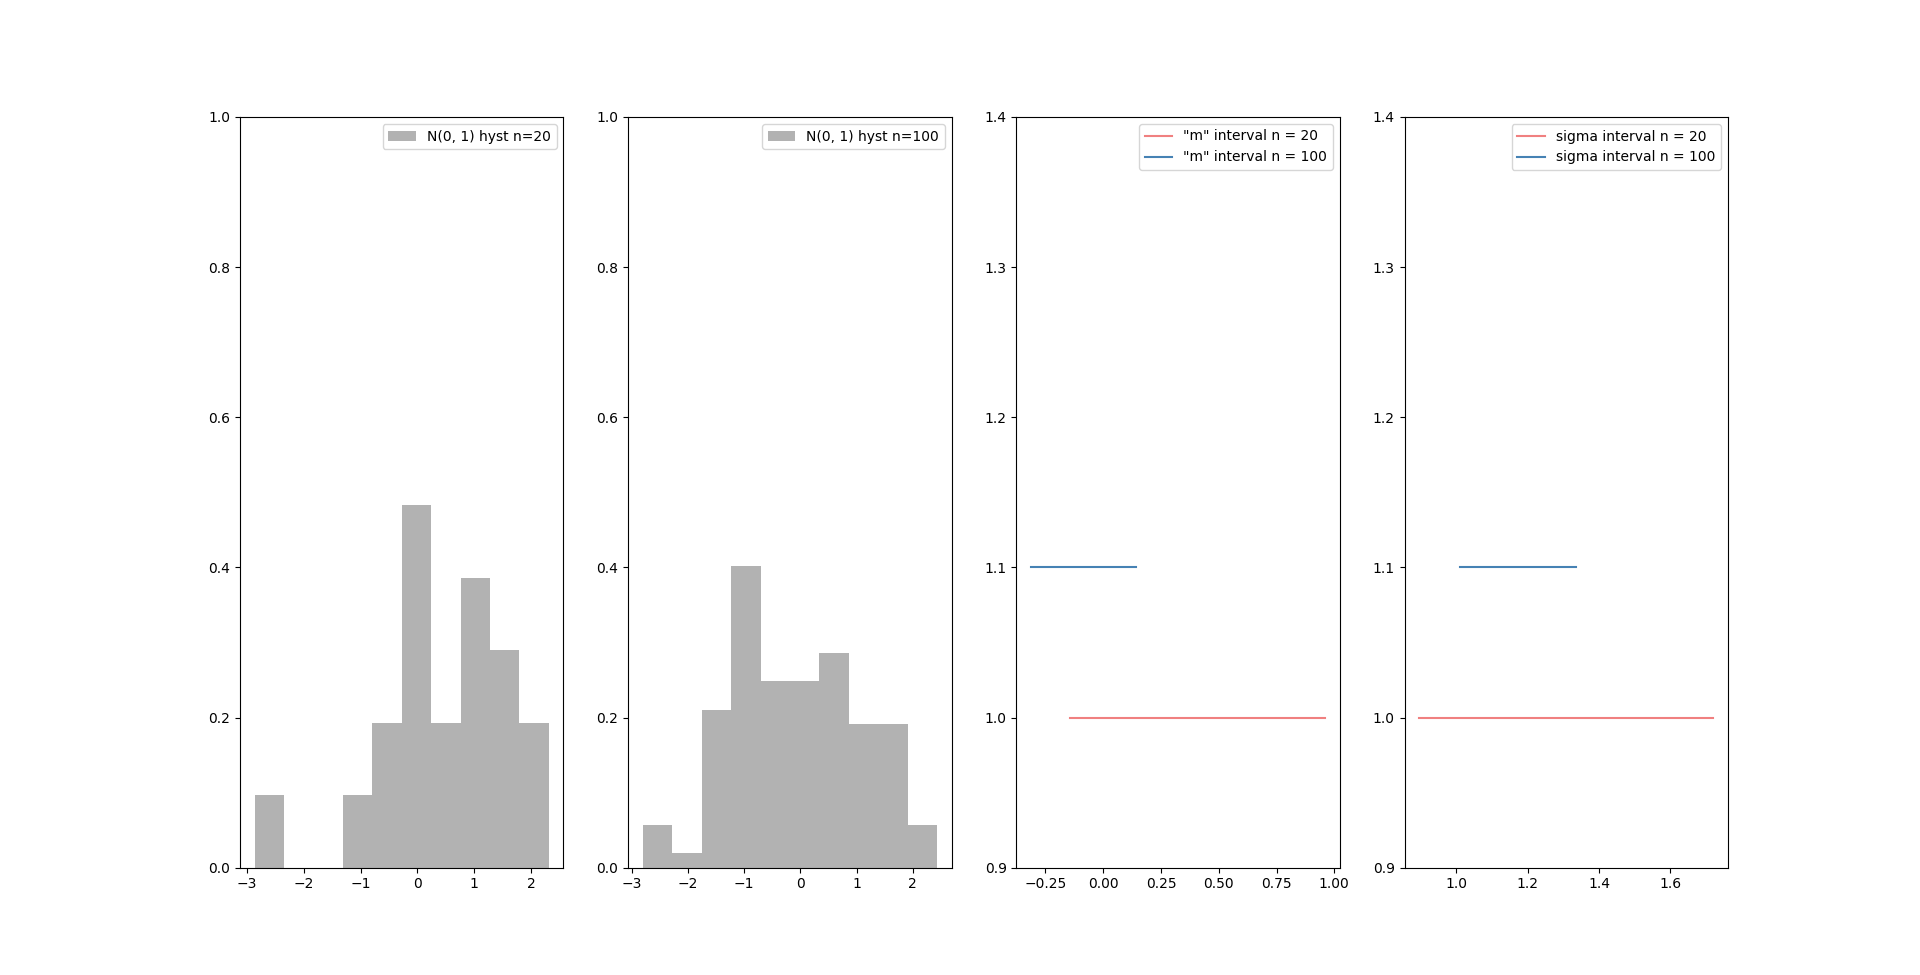
\includegraphics[width = 18cm, height = 6cm]{resources/8_1.png}
	\caption{Гистограммы нормальных распределений и доверительные интервалы их параметров}
	\label{w_pert}
\end{figure}

\begin{table}[H]
	\centering
	\begin{tabular}{| c | c | c |}
		\hline
		n = 20   &  $m$  & $\sigma$\\ \hline
		&  -0.14 < $m$ < 0.96 & 0.90 < $\sigma$ < 1.72 \\ \hline
		&   &   \\ \hline
		n = 100   &  $m$  & $\sigma$\\ \hline
		& -0.31 < $m$ < 0.14 & 1.01 < $\sigma$ < 1.34 \\
		\hline
	\end{tabular}
	\caption{Доверительные интервалы для параметров нормального распределения}
	\label{tab:interv_simple}
\end{table}

\subsection{Доверительные интервалы для параметров произвольного распределения. Асимптотический подход}
\begin{figure}[H]
	\centering
	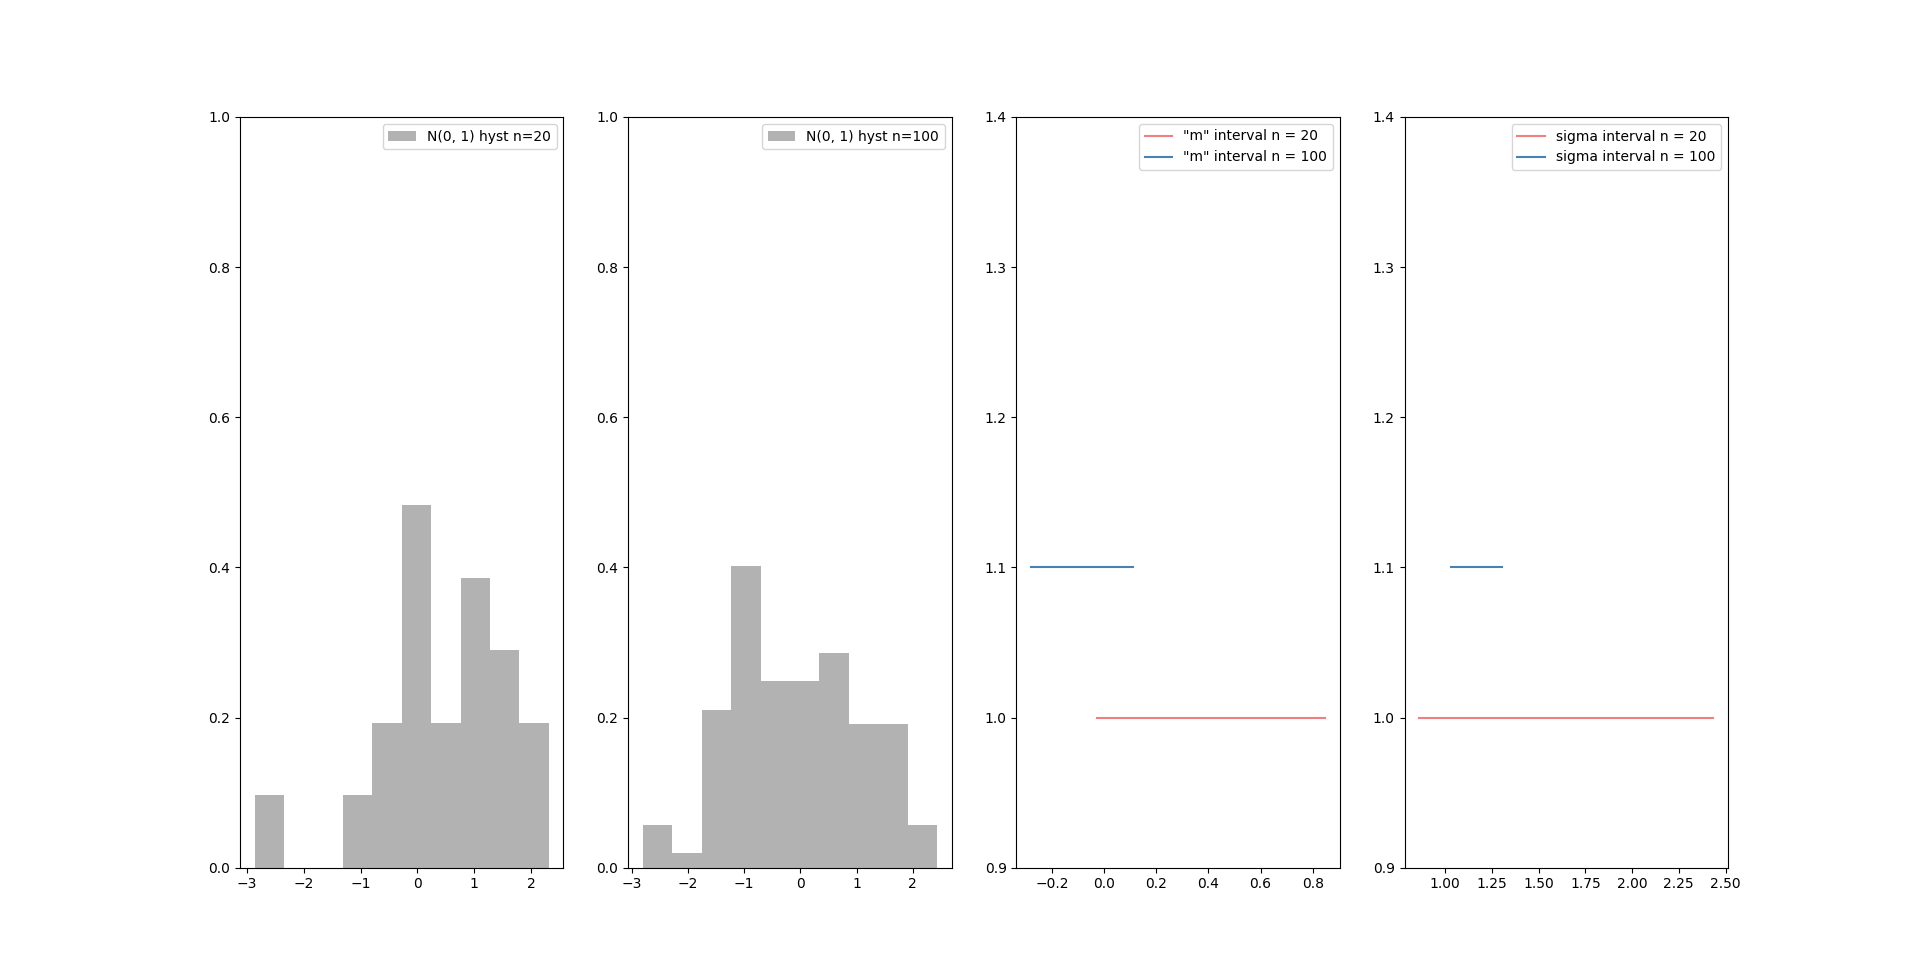
\includegraphics[width = 18cm, height = 6cm]{resources/8_2.png}
	\caption{Гистограммы нормальных распределений и доверительные интервалы их параметров. Асимптотический подход}
	\label{w_pert}
\end{figure}

\begin{table}[H]
	\centering
	\begin{tabular}{| c | c | c |}
		\hline
		n = 20   &  $m$  & $\sigma$\\ \hline
		&  -0.03 < $m$ < 0.85 & 0.86 < $\sigma$ < 2.43 \\ \hline
		&   &   \\ \hline
		n = 100   &  $m$  & $\sigma$\\ \hline
		& -0.28 < $m$ < 0.11 & 1.03 < $\sigma$ < 1.30 \\
		\hline
	\end{tabular}
	\caption{Доверительные интервалы для параметров произвольного распределения. Асимптотический подход}
	\label{tab:interv_asimpt}
\end{table}

\newpage